\documentclass{article}
\usepackage{graphicx}
\usepackage{float}
\usepackage{titlesec}
\usepackage{datetime}
\usepackage{geometry}
\usepackage{minted}
\usepackage{placeins}
\usepackage{caption}
\usepackage[document]{ragged2e}
\usepackage[hidelinks]{hyperref}
\usepackage{enumitem}
\geometry{
 a4paper,
 left=25mm,
 top=25mm,
 }
\captionsetup{hypcap=false} 
\newdateformat{daymonthyear}{\THEDAY .\THEMONTH .\THEYEAR}
\title{
  \centering
  
\includegraphics[width=\textwidth]{images/logo_PWr_kolor_poziom.png}\\
  \fontsize{28pt}{30pt}\selectfont Sprawozdanie 1\\
  % \fontsize{14pt}{30pt}\selectfont Ćwiczenie 1.
  }
\author{Krzysztof Zalewa}
\date{\daymonthyear\today}
\renewcommand*\contentsname{Spis treści}
\renewcommand{\figurename}{Rysunek}
\renewcommand{\listingscaption}{Skrypt}
\begin{document}
    \maketitle
    \pagebreak
    \tableofcontents
    \FloatBarrier
    \section{Cel skryptu}
      Celem zadania było napisanie trywialnego skryptu wypisującego tekst przy użyciu echo.
      Skrypt musi się wykonać, więc musi mieć ustawione prawa dostępu. Ponad to skrypt powinien 
      się wykonywać po wpisaniu jego nazwy (bez ścieżki).
    \section{Opis skryptu}
      \begin{frame}
        \scriptsize
        \inputminted[
            style={vs},
            breaklines,
            breakanywhere, 
            linenos, 
            tabsize=4 
        ]{bash}{../Skrypty/lab1.sh}
        \vspace{1em}
        \captionof{listing}{Główny skrypt}
        \label{lst:Maincode}
      \end{frame}
      \FloatBarrier
      \begin{figure}[ht]
        \centering
        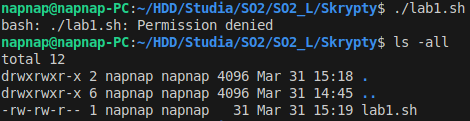
\includegraphics[width=\textwidth]{images/permission_denied.png}
        \caption{Odmowa wykonania skryptu}
        \label{fig:perm_denied}
      \end{figure}
      \FloatBarrier
      Samo napisanie skryptu nie wystarczy. Ponieważ domyślnie pliki nie mają praw do wykonywania się (Jak widać na
      (\hyperref[fig:perm_denied]{Rysunku \ref{fig:perm_denied}})). Problem ten można rozwiązać przy użyciu komendy
      \textbf{chmod +x nazwa\_skryptu}(Np. na \hyperref[fig:perm_granted]{Rysunku \ref{fig:perm_granted}})
      \begin{figure}[ht]
        \centering
        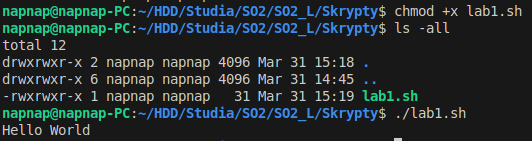
\includegraphics[width=\textwidth]{images/permission_granted.png}
        \caption{Skrypt wykonany}
        \label{fig:perm_granted}
      \end{figure}
      \FloatBarrier
      \raggedright
      Jednakże skryptu nie można jeszcze uruchomić przy pomocy nazwy. Nadal potrzeba ścieżki
      (\hyperref[fig:run_failed]{Rysunku \ref{fig:run_failed}}). Żeby komedna zadziałała zminennej PATH (ang. ścieżka)
      należy dodać ścieżkę do katalogu w którym jest skrypt (Tutaj PWD ang. print working directory). Następnie wykonanie 
      skryptu przy pomocy samej nazyw będzie możliwe (\hyperref[fig:run_succes]{Rysunku \ref{fig:run_succes}})
      \begin{figure}[ht]
        \centering
        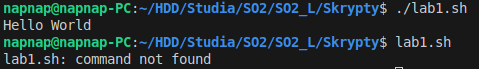
\includegraphics[width=\textwidth]{images/run_failed.png}
        \caption{Skrypt nie może zostać wykonany bez ścieżki}
        \label{fig:run_failed}
      \end{figure}
      \begin{figure}[ht]
        \centering
        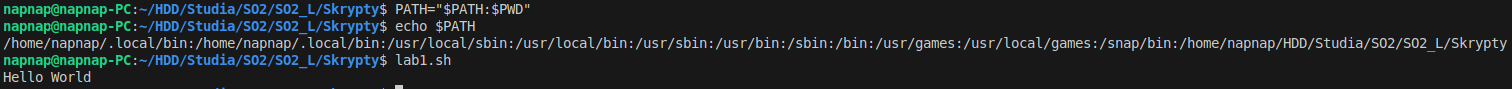
\includegraphics[width=\textwidth]{images/run_succes.png}
        \caption{Skrypt nie może zostać wykonany bez ścieżki}
        \label{fig:run_succes}
      \end{figure}
    \section{Wnioski}
      Skrypt wykonuje się poprawnie. Zadanie było trywialne. Jednakże stanowić będzie ono dobrą podstawę 
      do przyszłych zadań.
    \section{Źródła}
      \begin{enumerate}[label=\arabic*.]
        \item \url{https://www.geeksforgeeks.org/bash-scripting-introduction-to-bash-and-bash-scripting/}
      \end{enumerate}
\end{document}